\section{Introduction}
\label{sec:introduction}

% state the learning objective 
The objective of this laboratory assignment is to study a circuit containing:
\begin{itemize}
 \item 7 resistors $R_i$;
 \item a voltage source $V_S$ (with linear behaviour when t$<$0 and sinusoidal behaviour when t$\geq$0);
 \item a voltage controlled current source $I_b$;
 \item a current controlled voltage source $V_d$;
 \item a capacitor C.
\end{itemize}

\begin{figure}[h] \centering
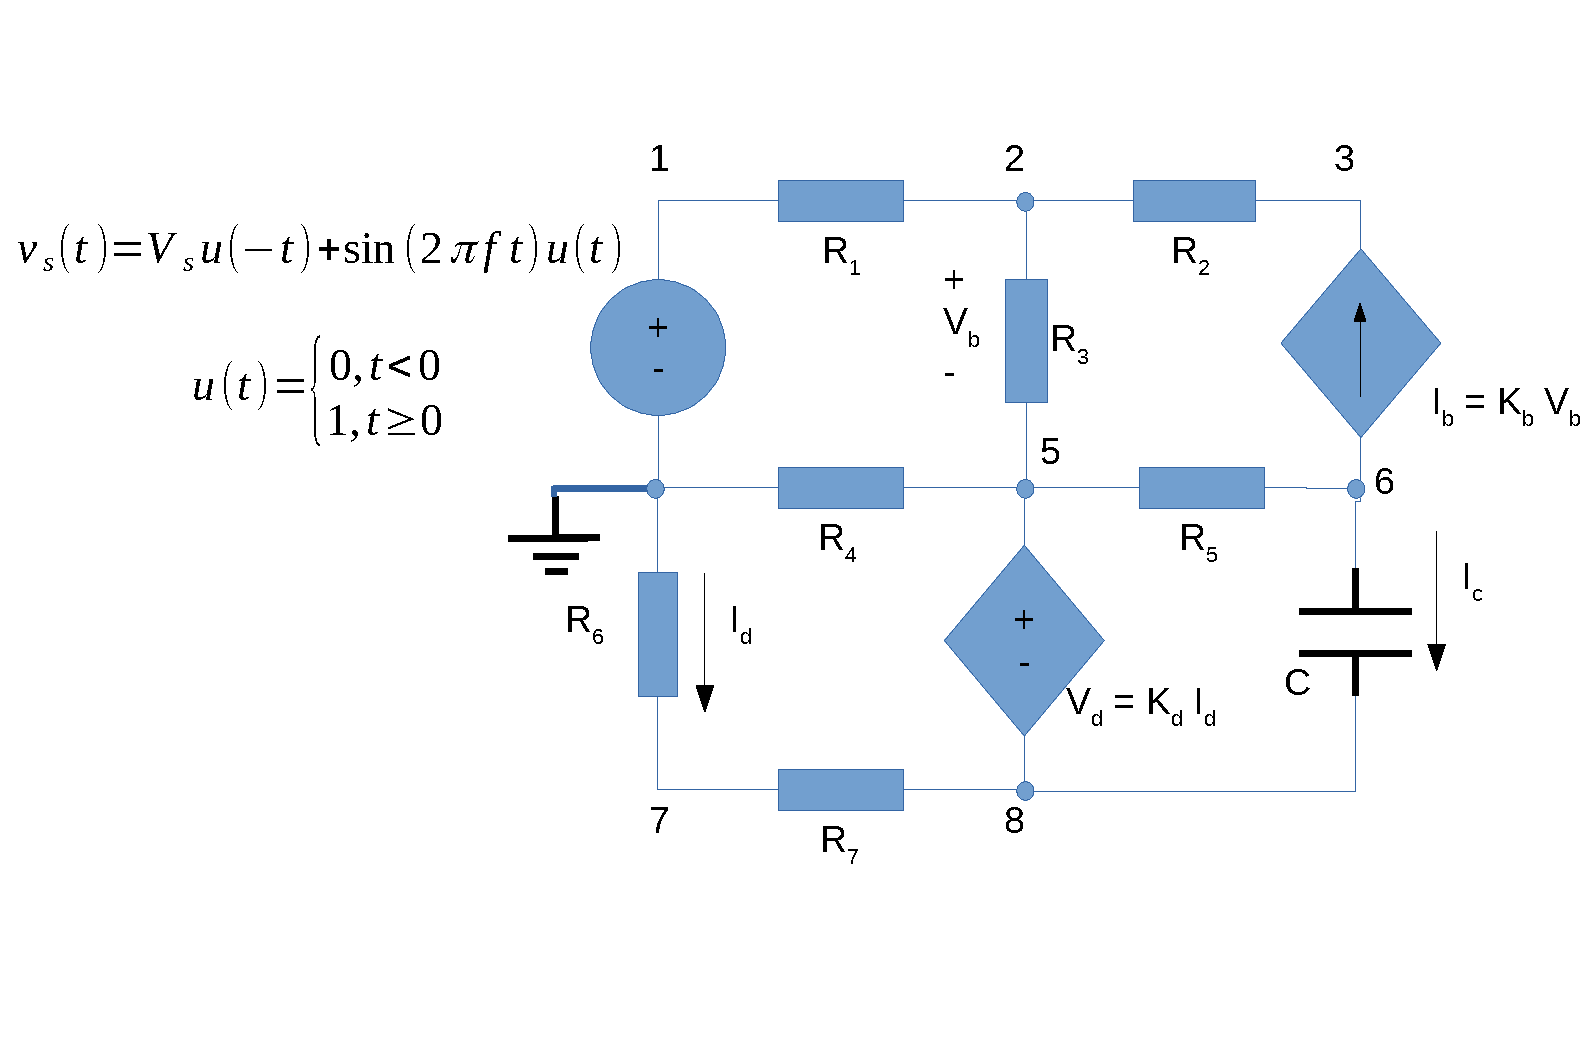
\includegraphics[width=0.8\linewidth]{rc.pdf}
\caption{The circuit under analysis}
\label{fig:rc}
\end{figure}

In Section \ref{sec:analysis}, a theoretical analysis of the circuit is
presented, following a series of steps. In Section\ref{sec:simulation}, the circuit is analysed by
simulation, and the results are compared to the theoretical results obtained in
Section~\ref{sec:analysis}. The conclusions of this study are outlined in
Section~\ref{sec:conclusion}.





